% !TeX spellcheck = it_IT

\section{Algoritmi probabilistici}

Cambia la \textbf{nozione di algoritmo}, oltre all'input del problema l'algoritmo è in grado di leggere da una \textbf{sorgente di bit casuali} (0 o 1 con pari probabilità). Sostanzialmente, una DTM con accesso anche a un nastro casuale utilizzabile quando necessario.\\

L'\textbf{output} quindi non è più deterministico, ma una \textbf{distribuzione di probabilità che dipende dall'input}. Anche il \textbf{tempo di esecuzione} diventa una \textbf{distribuzione} in base all'input.\\

Aggiungiamo un \textbf{componente probabilistico} agli algoritmi. L'output è diventa completamente deterministico se potessimo fissare i bit generati dalla componente casuale.\\

Nessun computer è in grado di simulare veramente una sorgente random, in quanto macchine deterministiche. Senza congegni strani ci si accontenta di \textbf{generatori pseudo-casuali PRNG}, ovvero una sequenza che sembra casuale ma che parte da un seed, e quindi riproducibile. Creano sequenze deterministiche che \textit{sembrano} casuali.\\

\newpage

\subsection{Problema del Taglio Minimo Globale (MinCut)}

Definizione:
\begin{itemize}
	\item \textbf{Input}: un grafo non orientato $G = (V,E)$
	\item \textbf{Soluzione ammissibile}: insieme di vertici $X \subseteq V$, con $X \neq \emptyset$ e che non deve avere complemento vuoto $X^C \neq \emptyset$ (dividere i vertici in due gruppi)
	\item \textbf{Funzione obiettivo}: l'insieme dei lati che hanno un'estremità in $X$ ed una estremità nel complemento di $X$
	$$ \{e \in E | e \cap X \neq \emptyset, e \cap X^C \neq \emptyset \} $$
	i.e., lati facente parti del taglio
	\item \textbf{Tipo}: minimizzazione $\min$
\end{itemize}

Si tratta di un problema $ \in \mathcal{NPO}c$.\\

Un \textbf{taglio} è una partizione dei vertici di un grafo $V$ in due sottoinsiemi disgiunti $S, T$. Gli archi che collegano un vertice di $S$ a uno di $T$ formano il taglio. Un taglio è \textbf{minimo} se il suo peso è minimo rispetto a tutti gli altri possibili tagli (insieme di lati più piccolo possibile).\\

\paragraph{Lemma:} Il taglio minimo è $\leq$ grado minimo.\\

Il taglio può essere al minimo 1, nel caso di un ponte tra due gruppi di nodi. Al massimo può essere il grado minimo in quanto basta tagliare quel numero di lati per dividere un nodo da tutti gli altri.\\

\newpage

\subsubsection{Algoritmo di Karger}

\paragraph{Contrazione di un grafo su un lato $e$:} Partendo da un grafo sul quale è presente un lato $e$ legato ai vertici $u$ e $v$, una contrazione si ottiene rimuovendo $e$ e facendo coincidere $u$ e $v$. \\

Da notare che se un terzo vertice $x$ è collegato sia a $u$ che a $v$, allora bisogna collegare con due archi il vertice risultato della contrazione $\{u,v\}$ a $x$. Contrarre un lato che ha dei "paralleli" vuol dire contrarre anche quest'ultimi.\\

Indichiamo la contrazione di $e$ su $G$ con $G \downarrow e$.\\

\textbf{Passaggi} dell'algoritmo:
\begin{itemize}
	\item Se $G$ non è connesso, emetti una componente connessa qualunque
	\item Altrimenti, finché ci sono più di 2 vertici, scegli un \textbf{lato casuale} e \textbf{contrai}
	\item Emetti la \textbf{classe di equivalenza} di uno dei due vertici
\end{itemize}

I due gruppi risultanti dal taglio corrisponderanno ai due gruppi di vertici "compressi" e i lati da tagliare saranno i vertici presenti tra quei gruppi di nodi.\\

\newpage

\paragraph{Esempio:} Grafo $G$
\begin{center}
	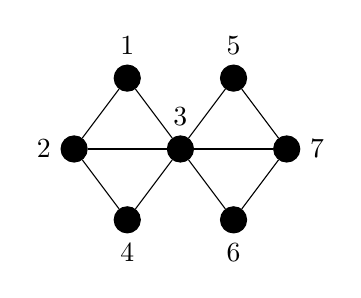
\begin{tikzpicture}[scale=0.45]
		\node[draw, circle, fill=black, label=90:1] (1) at (0,0) {};
		\node[draw, circle, fill=black, label=180:2] (2) at (-1.5,-2) {};
		\node[draw, circle, fill=black, label=90:3] (3) at (1.5,-2) {};
		\node[draw, circle, fill=black, label=270:4] (4) at (0,-4) {};
		\node[draw, circle, fill=black, label=90:5] (5) at (3,0) {};
		\node[draw, circle, fill=black, label=270:6] (6) at (3,-4) {};
		\node[draw, circle, fill=black, label=0:7] (7) at (4.5,-2) {};
		
		\draw[-] (1) to node {} (2);
		\draw[-] (1) to node {} (3);
		\draw[-] (2) to node {} (3);
		\draw[-] (2) to node {} (4);
		\draw[-] (3) to node {} (4);
		\draw[-] (3) to node {} (5);
		\draw[-] (3) to node {} (6);
		\draw[-] (3) to node {} (7);
		\draw[-] (5) to node {} (7);
		\draw[-] (6) to node {} (7);
		
	\end{tikzpicture}

	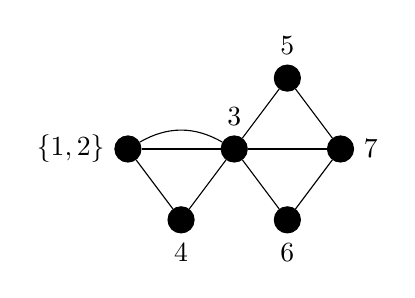
\begin{tikzpicture}[scale=0.45]
		\node[draw, circle, fill=black, label=180:{$\{1,2\}$}] (2) at (-1.5,-2) {};
		\node[draw, circle, fill=black, label=90:3] (3) at (1.5,-2) {};
		\node[draw, circle, fill=black, label=270:4] (4) at (0,-4) {};
		\node[draw, circle, fill=black, label=90:5] (5) at (3,0) {};
		\node[draw, circle, fill=black, label=270:6] (6) at (3,-4) {};
		\node[draw, circle, fill=black, label=0:7] (7) at (4.5,-2) {};
		
		\draw[-, bend left] (2) to node {} (3);
		\draw[-] (2) to node {} (3);
		\draw[-] (2) to node {} (4);
		\draw[-] (3) to node {} (4);
		\draw[-] (3) to node {} (5);
		\draw[-] (3) to node {} (6);
		\draw[-] (3) to node {} (7);
		\draw[-] (5) to node {} (7);
		\draw[-] (6) to node {} (7);
		
	\end{tikzpicture}
	
	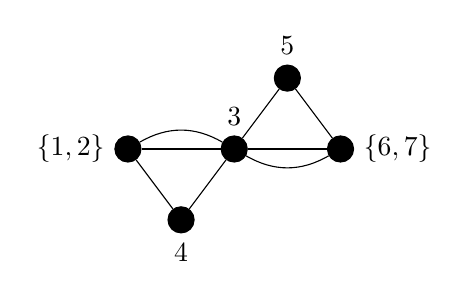
\begin{tikzpicture}[scale=0.45]
		\node[draw, circle, fill=black, label=180:{$\{1,2\}$}] (2) at (-1.5,-2) {};
		\node[draw, circle, fill=black, label=90:3] (3) at (1.5,-2) {};
		\node[draw, circle, fill=black, label=270:4] (4) at (0,-4) {};
		\node[draw, circle, fill=black, label=90:5] (5) at (3,0) {};
		\node[draw, circle, fill=black, label=0:{$\{6,7\}$}] (7) at (4.5,-2) {};
		
		\draw[-, bend left] (2) to node {} (3);
		\draw[-] (2) to node {} (3);
		\draw[-] (2) to node {} (4);
		\draw[-] (3) to node {} (4);
		\draw[-] (3) to node {} (5);
		\draw[-, bend right] (3) to node {} (7);
		\draw[-] (3) to node {} (7);
		\draw[-] (5) to node {} (7);
		
	\end{tikzpicture}
	
	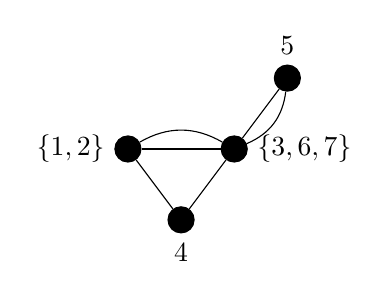
\begin{tikzpicture}[scale=0.45]
		\node[draw, circle, fill=black, label=180:{$\{1,2\}$}] (2) at (-1.5,-2) {};
		\node[draw, circle, fill=black, label=0:{$\{3,6,7\}$}] (3) at (1.5,-2) {};
		\node[draw, circle, fill=black, label=270:4] (4) at (0,-4) {};
		\node[draw, circle, fill=black, label=90:5] (5) at (3,0) {};
		
		\draw[-, bend left] (2) to node {} (3);
		\draw[-] (2) to node {} (3);
		\draw[-] (2) to node {} (4);
		\draw[-] (3) to node {} (4);
		\draw[-] (3) to node {} (5);
		\draw[-, bend left] (5) to node {} (3);
		
	\end{tikzpicture}
	
	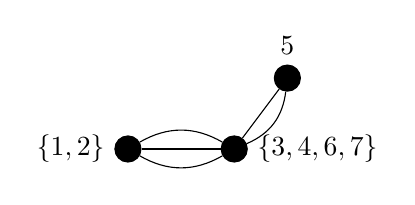
\begin{tikzpicture}[scale=0.45]
		\node[draw, circle, fill=black, label=180:{$\{1,2\}$}] (2) at (-1.5,-2) {};
		\node[draw, circle, fill=black, label=0:{$\{3,4,6,7\}$}] (3) at (1.5,-2) {};
		\node[draw, circle, fill=black, label=90:5] (5) at (3,0) {};
		
		\draw[-, bend left] (2) to node {} (3);
		\draw[-] (2) to node {} (3);
		\draw[-, bend left] (3) to node {} (2);
		\draw[-] (3) to node {} (5);
		\draw[-, bend left] (5) to node {} (3);
		
	\end{tikzpicture}
	
	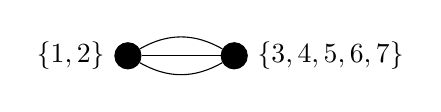
\begin{tikzpicture}[scale=0.45]
		\node[draw, circle, fill=black, label=180:{$\{1,2\}$}] (2) at (-1.5,-2) {};
		\node[draw, circle, fill=black, label=0:{$\{3,4,5,6,7\}$}] (3) at (1.5,-2) {};
		
		\draw[-, bend left] (2) to node {} (3);
		\draw[-] (2) to node {} (3);
		\draw[-, bend left] (3) to node {} (2);
		
	\end{tikzpicture}
\end{center}

Quindi possiamo dividere i vertici in $X = \{1,2\}$ e $X^C = \{3,4,5,6,7\}$ tagliando, nel grafo originale i lati $(1,3), (2,3),(2,4)$.

\newpage

Questo algoritmo \textbf{può ottenere la soluzione ottima}, ma anche \textbf{soluzioni arbitrariamente brutte}, non è un algoritmo di approssimazione, è \textbf{probabilistico}, potrebbe trovare qualcosa di molto lontano dall'ottimo, l'importante è che ci sia anche una probabilità di trovare quest'ultimo. Dobbiamo dimostrare che è presente una probabilità positiva di ottenere l'ottimo.\\

\begin{proof}
	Chiamiamo il grafo iniziale $G_1$ e $G_i$ il grafo prima dell'$i$-esima iterazione
	$$ G = G_1 \xrightarrow{G_1 \downarrow e_1} G_2 \xrightarrow{G_2 \downarrow e_2} \, \dots $$
	
	Chiamiamo $X^\ast$ il taglio minimo e $k^\ast$ la dimensione di quest'ultimo.\\
	
	\paragraph{Osservazioni:}
	\begin{enumerate}
		\item $G_i$ ha $n-i+1$ vertici (contrarre riduce i vertici sempre di 1)
		\item $G_i$ ha $\leq m -i+1$ lati dato che ne cancelliamo almeno 1 (potrebbero esserci paralleli) ogni volta
		\item Ogni taglio di $G_i$ corrisponde a un taglio di $G$ con la stessa dimensione
		\item Quindi il grado minimo di $G_i$ è $\geq k^\ast$, altrimenti (come visto nel Lemma) il taglio minimo non sarebbe davvero minimo
		\item Se $m_i$ sono i lati di $G_i$
		$$ 2 m_i = \sum_{v \in V_{G_i}} d_{G_i} (v)$$
		sarà pari alla metà della somma dei gradi di tutti i vertici, che a sua volta (per l'osservazione precedente)
		$$ \implies 2m_i \geq k^\ast (n-i+1) \implies m_i \geq \frac{k^\ast (n-i+1)}{2} $$
	\end{enumerate}
	
	Chiamando l'evento $E_i =$ "all'$i$-esima contrazione non contraiamo uno dei lati tagliati dal taglio minimo" (quindi dalla soluzione ottima).\\
	
	\newpage
	
	\paragraph{Lemma: }
	$$P[E_i | E_1, \, \dots \, , E_{i-1}] \geq \frac{n-i-1}{n-i+1}$$
	
	Dove la prima parte rappresenta la probabilità di togliere all'$i$-esimo passaggio uno dei lati necessari per il taglio minimo, dopo aver avuto la fortuna che ciò non sia accaduto per i primi $i-1$ passi.\\
	
	Di conseguenza: 
	\begin{flalign*}
		P[E_i | E_1, \, \dots \, , E_{i-1}]  
		& = 1 - P[\overline{E}_i | E_1, \, \dots \, , E_{i-1}]  \\
		& = 1 - \frac{k^\ast}{m_i}  \\
		& \geq 1 - \frac{k^\ast \cdot 2}{k^\ast (n-i+1)} \\ 
		& = \frac{n-i-1}{n-i+1}
	\end{flalign*}
	Quindi questa è la probabilità che all'$i$-esimo passo io non ho mai escluso nessuno dei lati necessari per il taglio minimo.\\
\end{proof}

\newpage

\addcontentsline{toc}{subsubsection}{\protect\numberline{}Teorema}
\paragraph{Teorema:} L'algoritmo di Karger emette il \textbf{taglio minimo} con \textbf{probabilità} 
$$\geq \frac{1}{\left(\begin{array}{c} n \\ 2 \end{array}\right)}$$

\begin{proof} Sapendo che 
	$$ P[E_1 \wedge E_2 \wedge \, \dots \, \wedge E_{n-1}] 
	= P[E_1] \cdot P[E_2 | E_1] \cdot \, \dots \, \cdot P [E_{n-2} | E_1, \, \dots \, , E_{n-3}]
	$$
	Per la proprietà della catena di eventi. Ma ognuna di quelle probabilità è nota, per il Lemma:
	\begin{flalign*}
		\geq \frac{n-2}{n} \cdot \frac{n-3}{n-1} \cdot \frac{n-4}{n - 2} \cdot \, \dots \, \cdot \frac{1}{3} 
		& = \frac{(n-2)! 2}{n!} \\ 
		& = \frac{2}{n(n-1)} \\ 
		& = \frac{1}{\left(\begin{array}{c} n \\ 2 \end{array}\right)} \\
	\end{flalign*}
\end{proof}

Quindi una probabilità relativamente piccola, che scala molto in fretta con $n$, ma \textbf{positiva}.\\

\newpage

\paragraph{Corollario:} Eseguendo l'algoritmo di Karger $\left(\begin{array}{c} n \\ 2 \end{array}\right) \ln n$ volte si ottiene il taglio minimo con probabilità $\geq 1 - \frac{1}{n}$ (possiamo dire "quasi certo", dato che tende ad $1$ per $n \rightarrow +\infty$).\\

\begin{proof}
	Dimostrazione: Sapendo che $\forall x >1$
	$$ \frac{1}{4} \leq1 - \left( 1 - \frac{1}{x}\right)^x \leq \frac{1}{e}$$
	
	Qual è la probabilità di NON trovare mai l'ottimo? Sarà
	$$ \leq \left(1 - \frac{1}{\left(\begin{array}{c} n \\ 2 \end{array}\right)}\right)^{\left(\begin{array}{c} n \\ 2 \end{array}\right) \ln n} 
	\leq \left(\frac{1}{e}\right)^{\ln n} 
	= \frac{1}{n}
	$$
\end{proof}

Quindi, eseguendo un algoritmo probabilistico che ha tempo polinomiale un numero polinomiale di volte ho sempre tempo polinomiale come risultato, ma sono \textit{quasi} certo di ottenere l'ottimo.\\

Se eseguo tante volte un algoritmo che può darmi soluzioni molto brutte, ma potenzialmente anche l'ottimo, prima o poi qualcosa di buono lo trovo.\\

% End L14

\newpage

\addcontentsline{toc}{subsection}{\protect\numberline{}\textit{Cose}}
\subsection*{\textit{Cose}}

Una serie di \textit{Cose}$^\text{\textregistered}$ che potrebbero essere utili: 

\begin{enumerate}
	\item \textbf{Chain rule (regola della catena):} la probabilità della congiunzione di eventi si può sempre esprimere come probabilità del primo per probabilità del secondo dato il primo, fino all'ultimo
	$$ P[E_1 \wedge E_2 \wedge \, \dots \, \wedge E_n] = P [E_1] \cdot P [E_2 | E_1] \cdot \, \dots \, \cdot P[E_n | E_1 \, \dots \, E_{n-1}] $$
	
	\item $\forall x > 1$
	$$ \frac{1}{4} \leq \left(1 - \frac{1}{x}\right)^x \leq \frac{1}{e} $$
	
	\item \textbf{Union bound:} la probabilità dell'unione di eventi è minore della somma di probabilità degli eventi (uguale solo se sono tutti disgiunti):
	$$ P\left[ \bigcup_i E_i \right] \leq \sum_i P[E_i] $$
	
	\item \textbf{Disuguaglianza di Markov:} avendo una variabile aleatoria $x$ non negativa e con media finita e un $\alpha > 0$, allora
	$$ P[x \geq \alpha] \leq \frac{E[x]}{\alpha} $$
	la probabilità che $x$ sia maggiore di $\alpha$ è minore uguale della media di $x$ diviso $\alpha$.
	
	\item $\forall x \in [0,1]$
	$$ 1 - x \leq e^{-x} $$
	
	\item \textbf{Teorema delle probabilità totali:} la probabilità di un evento può essere calcolata sommando le probabilità condizionate di tale evento rispetto a un insieme completo di eventi mutuamente esclusivi.\\
\end{enumerate}

\newpage

\subsection{Problema SetCover}

Già visto, per più informazioni guarda il \hyperref[subsec:setcover]{\texttt{capitolo a riguardo}}.\\

\textbf{Definizione}:
\begin{itemize}
	\item \textbf{Input}: $S_0, \, \dots \, , S_{m-1}$, con $\bigcup_{i \in m} = U$ con pesi $w_o, \, \dots \, , w_{m-1} \in Q^+$
	
	\item \textbf{Soluzioni ammissibili}: $I \subseteq m$ tale che
	$$ \bigcup_{i \in I} S_i = U $$
	
	\item \textbf{Funzione obiettivo}: 
	$$ w = \sum_{i \in I} w_i $$
	
	\item \textbf{Tipo}: minimizzazione, $\min$
\end{itemize} 

Chiamo $n:= |U|$ la \textbf{cardinalità dell'universo}.\\

Si può formulare come un \textbf{problema di programmazione lineare intera ILP}. Prendo $x_0, \, \dots \, , x_{m-1}$ variabili, ognuna di queste dice se includere o meno il relativo insieme. La funzione da minimizzare è 
$$ w_0 x_0 + w_1 x_1 + \, \dots \, + w_n x_n $$

Quindi i vincoli sono:
$$ 
\begin{cases}
	0 \leq x_j \leq 1 & \forall j \in n \\
	\sum_{i: p \in S_i} x_i \geq 1  &\forall p \in U
\end{cases}
$$

La prima riga vuol dire che \textbf{ogni variabile può essere tra 0 e 1} (ma abbiamo solo valori interi), di conseguenza prendere o meno il set.\\
La seconda riga vuol dire che \textbf{almeno un insieme deve coprire ogni punto dell'universo}.\\

Risolvendo questo problema sugli interi si ottiene la soluzione ottima, ma si può rilassare su numeri reali per risolverlo (non ottimamente) in tempo polinomiale. Consideriamo $\hat \pi$ la \textbf{versione rilassata} di programmazione lineare non intera di questo problema.\\

\newpage

\subsubsection{Arrotondamento Aleatorio}

L'idea dietro l'algoritmo di arrotondamento aleatorio per SetCover è la seguente.

\begin{algorithm}
	\caption{ArrotondamentoAleatorioSetCover()}
	\begin{algorithmic}
		\STATE Costruiamo $\pi$
		\STATE Risolviamo la versione rilassata $\hat \pi$, ottenendo soluzione $\hat x$ (vettore di valori soluzione)
		\STATE $I \leftarrow \emptyset$
		\FOR{$i \in m$}
			\FOR{$t = 1, \, \dots \, , \lceil k + \ln n \rceil$}
				\STATE aggiungiamo $i$ a $I$ con probabilità $\hat x_i$ 
			\ENDFOR
		\ENDFOR
		\STATE Output $I$
	\end{algorithmic}
\end{algorithm}

Il \texttt{for} per l'inserimento può essere visto anche come: "Inserisci $i$ in $I$ con probabilità $1 - (1-\hat x_i)^{\left\lceil k + \ln n \right\rceil}$".\\

Usiamo la \textbf{soluzione} $\hat x_i$ \textbf{come probabilità}, più il valore è alto più è probabile che verrà inserito nella soluzione finale. $k$ è un parametro, dentro l'algoritmo, mentre $\alpha$ è esterno, scelto da noi.\\

Sebbene improbabile, \textbf{potrebbe non portare a una soluzione ammissibile}, che non copre tutto l'universo. Quando anche fornisce una soluzione ammissibile \textbf{non è detto che sia ottima}.\\

\newpage

\addcontentsline{toc}{subsubsection}{\protect\numberline{}Teorema}
\paragraph{Teorema:} L'algoritmo ha queste proprietà:
\begin{enumerate}
	\item Produce una \textbf{soluzione ammissibile con probabilità} $\geq 1 - e^{-k}$.\\
	
	\item Per ogni $\alpha > 0$, la \textbf{probabilità} che il \textbf{fattore di approssimazione} (quanto lontano dall'ottimo è la soluzione) sia $\geq \alpha (k + \ln n)$ è $\leq 1/\alpha$
	$$ P[\text{fatt. appr. } \geq \alpha (k + \ln n)] \leq \frac{1}{\alpha} $$
	Insomma, la probabilità che l'algoritmo vada male è bassa.\\
\end{enumerate}

\begin{proof}
	\textbf{Notazione}: ricordando come è fatto l'input (vedi sopra), risolvendo la versione $\hat \pi$ ottengo $\hat x_0, \, \dots \, , \hat x_{m-1} \in [0,1]$ e la soluzione del problema rilassato è 
	$$ \hat w = w_0 \hat x_0 + \, \dots \, + w_{m-1} \hat x_{m-1} $$
	
	E $w^\ast$ è la soluzione ottima, ovviamente $\hat w \leq w^\ast$.\\
	
	\textbf{Punto 1:} Probabilità che la soluzione sia ammissibile: chiamando 
	$$ E_p = \text{il punto } p \in U \text{ non è coperto} $$
	\begin{flalign*}
		P[\text{sol. amm.}] & = 1 - P[\text{sol. non amm.}]   \\
		& = 1 - P[\text{almeno un punto di } U \text{ non coperto}]  \\
		& = 1 - P\left[\bigcup_{p \in U} E_p  \right]  \geq 
	\end{flalign*}
	
	Usando l'union bound
	\begin{flalign*}
		& \geq 1 - \sum_{p \in U} P[E_p] \\
		& = 1 - \sum_{p \in U} P[p \text{ non è coperto}]\\
		& = 1 - \sum_{p \in U} \left( \prod_{i \in m, p \in S_i} P[i \text{ non è stato scelto}]\right)
	\end{flalign*}
	
	\newpage
	
	Quindi la probabilità che un punto non sia coperto è il prodotto delle probabilità di non aver scelto nessun insieme che lo contengo, e posso dire meglio quando questa cosa succede, per definizione dell'algoritmo:
	\begin{flalign*}
		& = 1 - \sum_{p \in U} \prod_{i \in m, p \in S_i} (1 - \hat x_i)^{\lceil k + \ln n \rceil}  \\
		& \geq 1 - \sum_{p \in U} \prod_{i \in m, p \in S_i} (1 - \hat x_i)^{k + \ln n} \geq
	\end{flalign*}
	
	Uso il fatto che $1-x \leq e^{-x}$:
	\begin{flalign*}
		& \geq 1 - \sum_{p \in U} \prod_{i \in m, p \in S_i} e^{- \hat x_i (k + \ln n)} \\
		& = 1 - \sum_{p \in U} e^{- (k + \ln n) \sum_{i \in m, p \in S_i} \hat x_i} \geq
	\end{flalign*}
	
	Ma uno dei vincoli delle LP per la seconda sommatoria è che questa sia $\geq 1$, quindi
	\begin{flalign*}
		& \geq 1- \sum_{p \in U} e^{-(k + \ln n)} \\ 
		& = 1 - \sum_{p \in U} \frac{1}{n} e^{-k}  \\
		& = 1 - e^{-k} \sum_{p \in U}  \frac{1}{n} \\
		& = 1 - e^{-k}
	\end{flalign*}
	Ricordando che $|U| = n$.\\
	
	\newpage
	
	\textbf{Punto 2:} La probabilità che $S_i$ venga scelto è $\leq (k + \ln n) \hat x_i$ (per union bound). Il valore atteso di $w$ è 
	\begin{flalign*}
		E[w] & = \sum_{i \in m} w_i P[S_i \text{ sia scelto}] \\
		& \leq \sum_{i \in m} w_i (k + \ln n) \hat x_i  \\
		& = (k + \ln n) \sum_{i \in m} w_i \hat x_i =
	\end{flalign*}
	Ma è la definizione di $\hat w$ quindi
	\begin{flalign*}
		& = (k + \ln n)\hat w \\
		& \leq (k + \ln n) w^\ast
	\end{flalign*}
	
	Vogliamo usare la disuguaglianza di Markov, scegliendo come parametro $\beta .= \alpha (k + \ln n) w^\ast$. Mi importa che
	$$ P\left[x \geq \beta\right] \leq \frac{E[x]}{\beta} $$
	
	Quindi
	\begin{flalign*}
		P \left[\frac{w}{w^\ast} \geq \alpha (k + \ln n) \right] & = P\left[w \geq \alpha (k + \ln n) w^\ast \right] \\
		& = P [w \geq \beta] \leq 
	\end{flalign*}
	
	Per la disuguaglianza di Markov
	\begin{flalign*}
		& \leq \frac{E[w]}{\beta} \\
		& \leq \frac{(k + \ln n) w^\ast}{\alpha (k + \ln n) w^\ast} \\
		& = \frac{1}{\alpha}
	\end{flalign*}
\end{proof}

\newpage

\paragraph{Corollario:} Per $k=3$, c'è il $45\%$ di \textbf{probabilità di ottenere una soluzione ammissibile con rapporto di approssimazione} $\leq 6 + 2 \ln n$.\\

\begin{proof}
	La probabilità che una soluzione sia non ammissibile è piccola, il resto delle volte la soluzione è ammissibile ma il rapporto di approssimazione non ci piace abbastanza.\\
	
	Quindi abbiamo uno spazio di soluzioni non ammissibili $E_{\text{non-amm}}$, delle soluzioni che non vogliamo $E_{\text{bad}}$ e le soluzioni che effettivamente ci vanno bene $E_{\text{ok}}$.\\
	
	La probabilità delle soluzioni non ammissibili è:
	$$ P[E_{\text{non-amm}}] \leq e^{-k} = e^{-3} $$
	
	Dal rapporto di approssimazione possiamo capire che $\alpha = 2$, quindi la probabilità per le soluzioni che non vogliamo è
	$$ P[E_{\text{bad}}] = P[\text{fatt. appr. } > 6 + 2 \ln n] \leq \frac{1}{2} $$
	
	Per le soluzioni buone invece:
	\begin{flalign*}
		P[E_{\text{ok}}] & = 1 - P[E_{\text{non-amm}} \cup E_{\text{bad}}] \\ 
		& \geq 1 - \left(P[E_{\text{non-amm}}] + P[E_{\text{bad}}]\right) \\
		& \geq 1 - \left(e^{-3} + \frac{1}{2}\right) \approx 45\%
	\end{flalign*}
\end{proof}

% End L15

\newpage

\subsection{Problema MaxEkSat}

Dove $k$ è un parametro $\geq 3$.\\

\textbf{Definizione}: 
\begin{itemize}
	\item \textbf{Input}: una formula CNF in cui ogni clausola contiene esattamente $k$ letterali
	\item \textbf{Soluzioni Ammissibili}: assegnamenti di valori di verità (per le variabili che compaiono nell'input)
	\item \textbf{Funzione obiettivo}: numero di clausole soddisfatte
	\item \textbf{Tipo}: massimizzazione, $\max$
\end{itemize}

Ovviamente è $\mathcal{NPO}$, in quanto facilmente riconducibile a un SAT generico.\\


\subsubsection{Algoritmo Probabilistico}

\textbf{Passaggi}: 
\begin{itemize}
	\item Assegna a ogni variabile un valore a caso $\in \{true, false\}$
\end{itemize}

\addcontentsline{toc}{subsubsection}{\protect\numberline{}Teorema}
\paragraph{Teorema:} Questo algoritmo \textbf{rende vere} almeno 
$$ \frac{2^k-1}{2^k} = 1 - \frac{1}{2^k} $$
delle clausole totali.\\

Alternativamente, questo algoritmo, data una formula con $t$ clausole, ne \textbf{rende vere almeno}
$$ \frac{2^k-1}{2^k} t $$
Cioè 
$$ E[T] \geq  \frac{2^k-1}{2^k} t  $$

Un po' di \textbf{notazione:} sia $\varphi$ l'\textbf{input}, chiamiamo 
\begin{itemize}
	\item $n$ il numero di variabili che compaiono
	\item $k$ il numero di letterali per clausola 
	\item $x_1, \, \dots \, , x_n$ le variabili che compaiono nelle clausole
	\item $K_1, \, \dots \, , K_t$ le clausole
\end{itemize}

Variabili aleatorie: 
\begin{itemize}
	\item $x_i$: variabile uniforme in $(0,1)$, variabile che uso per decidere se rendere vera o falsa la variabile $i$-esima. Assegniamo 0 o 1 a caso per tutte
	\item $C_i$: variabile aleatoria che ha valore:
	$$ C_i = \begin{cases}
		1 & \text{ se } K_i \text{ soddisfatta } \\
		0 &  \text{ altrimenti }
	\end{cases}
	$$
	\item $T$: numero di clausole soddisfatte
\end{itemize}

\begin{proof}
	Qual è il \textbf{numero atteso di clausole soddisfatte} $E[T]$?
	\begin{flalign*}
		E[T] & = \sum_{b_1 \in \{0,1\}} \, \dots \, \sum_{b_n \in \{0,1\}} E [T | x_1 = b_1, \, \dots \, , x_n = b_n] P[x_1 = b_1, \, \dots \, , x_n = b_n] \\
		& =  \sum_{b_1 \in \{0,1\}} \, \dots \, \sum_{b_n \in \{0,1\}} E[C_1 + \, \dots \, + C_t | x_1 = b_1, \, \dots \, , x_n = b_n] P[x_1 = b_1] \, \dots \, P[x_n = b_n]
	\end{flalign*}
	
	Ma ognuna delle $n$ probabilità è $1/2$ (dato che l'assegnamento è casuale), quindi 
	$$
	= \frac{1}{2^n} \sum_{b_1 \in \{0,1\}} \, \dots \, \sum_{b_n \in \{0,1\}} E[C_1 + \, \dots \, + C_t | x_1 = b_1, \, \dots \, , x_n = b_n]
	$$
	
	Sostituisco alla probabilità il \textbf{valore atteso}:
	$$ 
	= \frac{1}{2^n} \sum_{b_1 \in \{0,1\}} \, \dots \, \sum_{b_n \in \{0,1\}} \sum_{j=1}^t E[C_j | x_1 = b_1, \, \dots \, , x_n = b_n]
	$$
	
	Dove, ogni clausola $K_j$ può essere falsa solo nel caso in cui ognuna delle variabili $x_i$ che la compone si presenta nella forma:
	\begin{itemize}
		\item $false$ se $x_i \in K_j$
		\item $true$ se $\neg x_i \in K_j$
	\end{itemize}
	
	%TODO: Chiedere/controllare
	Quindi c'è un singolo assegnamento che rende $K_j$ falsa, mentre ci sono $2^n - 2^{n-k}$ modi per renderla vera.\\ 
	
	Quindi la sommatoria sopra diventa
	$$ 
	= \frac{1}{2^n} \sum_{j=1}^t (2^n - 2^{n-k}) 
	= \frac{2^n - 2^{n-k}}{2^n} t 
	= \frac{2^{k-n} 2^n - 2^{k-n} 2^{n-k}}{2^{k-n} 2^n} t
	= \frac{2^k - 1}{2^k} t
	$$
	%End proof?
\end{proof}

%\newpage

\paragraph{Lemma:} Per ogni $j = 0, \, \dots \, , n$ esistono $b_1, \, \dots \, , b_j \in \{0,1\}$ tali che
$$ E[T |  x_1 = b_1, \, \dots \, , x_j = b_j] \geq \frac{2^k - 1}{2^k} t $$
dove $t$ è il numero di clausole.\\

\begin{proof}
	Per induzione su $j$:
	\begin{itemize}
		\item \textbf{Base:} Per $j=0$ è il teorema.\\
		
		\item \textbf{Passo induttivo:} per ipotesi di induzione
		$$\frac{2^k-1}{2^k} t \leq  E[T |  x_1 = b_1, \, \dots \, , x_{j-1} = b_{j-1}] = $$
		
		Per il teorema delle probabilità totali:
		\begin{flalign*}
			& = E[T | x_1 = b_1, \, \dots \, , x_{j-1} = b_{j-1}, x_j = 0] P[x_j = 0]  \\
			& \hspace*{3cm} + E[T | x_1 = b_1, \, \dots \, , x_{j-1} = b_{j-1}, x_j = 1] P[x_j = 1] \\
			& = \frac{1}{2} (E[T | x_1 = b_1, \, \dots \, , x_{j-1} = b_{j-1}, x_j = 0] \\ 
			& \hspace*{3cm} + E[T | x_1 = b_1, \, \dots \, , x_{j-1} = b_{j-1}, x_j = 1] )
		\end{flalign*}
		Ipotizzando che per assurdo i due valori siano: 
		$$ 
		E[T | x_1 = b_1, \, \dots \, , x_{j-1} = b_{j-1}, x_j = 0] < \frac{2^k-1}{2^k} t
		$$
		$$
		E[T | x_1 = b_1, \, \dots \, , x_{j-1} = b_{j-1}, x_j = 1] < \frac{2^k-1}{2^k} t
		$$
		Ma questo vorrebbe dire che la loro somma è
		$$ 
		< \frac{2^k - 1}{2^k} 2t 
		$$
		Ma questo va contro l'ipotesi induttiva, quindi almeno uno dei due deve essere $\geq$.\\
	\end{itemize}
\end{proof}

%L'algoritmo si riesce a derandomizzare ... %Wtf 

\paragraph{Corollario:} Esiste un \textbf{assegnamento deterministico che soddisfa almeno} 
$$ \frac{2^k - 1}{2^k} t$$
clausole.\\
Input: Formula $k$-CNF fatta da $t$ clausole $K_1 \wedge \, \dots \, \wedge K_t$ e $n$ variabili $x_1, \, \dots \, , x_n$.\\
Per capire come assegnarle.\\
\begin{algorithmic}
	\STATE $D \leftarrow \emptyset$
	\FOR{$i=1, \, \dots \, , n$}
		\STATE $\Delta_0 \leftarrow 0$, $\Delta_1 \leftarrow 0$
		\STATE $\Delta_{D_0} \leftarrow \emptyset$, $\Delta_{D_1} \leftarrow \emptyset$
		\FOR{$j = 1, \, \dots \, , t$}
			\IF{$j \in D$ \textbf{or} $x_i$ non compare in $K_j$}
				\STATE continue
			\ENDIF
			\STATE $h \leftarrow$ numero di variabili in $K_j$ con indice $\geq i$
			\IF{$x_i$ compare positiva in $K_j$}
				\STATE $\Delta_0 \leftarrow \Delta_0 - \frac{1}{2^h}$
				\STATE $\Delta_1 \leftarrow \Delta_1 + \frac{1}{2^h}$
				\STATE $\Delta_{D_1} \leftarrow \Delta_{D_1} \cup \{j\}$
			\ELSE
				\STATE $\Delta_0 \leftarrow \Delta_0 + \frac{1}{2^h}$
				\STATE $\Delta_1 \leftarrow \Delta_1 - \frac{1}{2^h}$
				\STATE $\Delta_{D_0} \leftarrow \Delta_{D_0} \cup \{j\}$
			\ENDIF
		\ENDFOR
		\IF{$\Delta_0 \geq \Delta_1$}
			\STATE $x[i] = false$
			\STATE $D \leftarrow D \cup \Delta_{D_0}$
		\ELSE
			\STATE $x[i] = true$
			\STATE $D \leftarrow D \cup \Delta_{D_1}$
		\ENDIF
	\ENDFOR
	\STATE Output $x[i], \, \dots \, x[n]$
\end{algorithmic}

\newpage

Questo algoritmo tenta di "mimare" quello visto nel Lemma, conoscendo un assegnamento "buono" delle prime $j$ variabili posso conoscere un assegnamento "buono" delle prime $j+1$.\\

Notazione:
\begin{itemize}
	\item $\Delta_1/\Delta_0$: valore atteso se viene posta ad 1 e a 0 la variabile, rispettivamente.\\
	
	\item $\Delta_{D_1}/\Delta_{D_0}$: l'insieme di clausole chiuse da un determinato assegnamento ($true$ o $false$ rispettivamente).\\
\end{itemize}

Per ogni variabile (\texttt{for} esterno), per ogni clausola (\texttt{for} interno) determina cosa succederebbe al valore atteso se assegnassi un certo valore di verità alla variabile (\texttt{if/else}, rispettivamente \textit{true/false}).\\

\vfill

(Non ho capito, ma farò finta)

\newpage

%End L16